\documentclass{article}
\usepackage[utf8]{inputenc}

\title{LIA project proposal: DAFFE\\Geographically Elastic Application \& Data Volume Migration Automation}
\author{Thijs Houtenbos  \\
\href{mailto:Mathijs.Houtenbos@os3.nl}{\texttt{Mathijs.Houtenbos@os3.nl}}\\[0.2cm] 
Nikolaos Petros Triantafyllidis\\
\href{mailto:Nikolaos.Triantafyllidis@os3.nl}{\texttt{Nikolaos.Triantafyllidis@os3.nl}}}

\date{\today}

\usepackage{graphicx}
\usepackage{hyperref}
\usepackage{framed}

\begin{document}

\maketitle

\section{Introduction}
The current way to globally serve an application while minimizing latencies is by replicating data around the globe. This, however, requires keeping data consistent which is no trivial task as it costs bandwidth and other computational resources.\\ \textbf{Then why not move the data to where it is needed the most?} Currently there is no automated way to migrate online applications together with their data, based on client geographical distribution. Implementing this technique may \textbf{reduce latency, bandwidth and overall cost}.\\
\\
We propose a solution to this problem by combining several existing software components to form a software stack. The functionality of some of these components needs to be extended by developing new modules. The desired result will be a new \textbf{automated technique of migrating applications including data} based on changing client geographical distribution, and testing if this has the desired effect.

% \pagebreak


\section{Components}

\begin{itemize}
    \item{\textbf{Docker}: Operating-system-level virtualization is a virtualization method where the OS kernel allows multiple isolated user spaces. Each user space instance is usually referred to as a  \textbf{Software-container} \cite{OSLV}.\\
\textbf{Docker} \cite{Docker} is a software platform that provides application deployment automation by packaging applications and their dependencies into lightweight software containers. At the same time Docker exposes a cloud service for sharing application containers and workflows between users \cite{whatisdocker}.}
    \item{\textbf{Anisble}: We propose a software stack that builds upon \textbf{Docker} and \textbf{Flocker}, to provide efficient application and data volume migration. The stack will be managed by \textbf{Ansible} \cite{ansible}, a lightweight and streamlined, open source configuration management tool that has build-in capabilities for a variety of everyday administration tasks. Ansible is easily extensible in a very straightforward manner \cite{ansiblemod}.} 
    \item{\textbf{Flocker}: While with \textbf{Docker} application portability becomes very easy, database migration and cluster provisioning is still a tricky task. A solution to this is provided by \textbf{Flocker} \cite{flocker}, a software tool that allows controlling of the data with the same tools as any stateless application. Flocker packages the data into Docker containers and moves them around nodes as any other application \cite{flockerdoc}.}
    \item{\textbf{Fig}: Fig is a tool for creating and running complex applications on Docker by defining multi-container applications in a single file \cite{fig}. Now integral part of Docker \cite{figgit}.}
    \item{\textbf{ELK}: Stands for \textbf{Elasticsearch}, \textbf{Logstash} and \textbf{Kibana}. An end-to-end stack that delivers real-time insights from structured and unstructured data sources \cite{elk}. ELK will provide us with the geographical data analytics which we will utilize to perform the data migrations in an efficient manner}
\end{itemize}
The project name DAFFE consists of the first letters of these 5 components.

\subsection{Component selection notes}
We have the option to choose between multiple  configuration management tools. We looked more thoroughly at two options: \textbf{Ansible} and \textbf{Foreman} \cite{foreman}. We chose Ansible over Foreman mostly because of simplicity, since Foreman builds on Puppet and Ruby-on-Rails\cite{foremandoc}. With Ansible writing a plugin is as simple as testing the concept by creating a Python script that executes the commands \cite{ansiblemod}. We might miss the centralized management that Foreman offers, but we can write some easy test scripts to provide centralization.\\
\\
Fig is explicitly mentioned (even though it is now a standard Docker tool) because it is used for fast and easy configuration allowing us to test and deploy multiple setups in the short timeframe for LIA. Another optional additional tool that can  help automate test setup that deserves mention is Vagrant \cite{vagrant}.

\section{Plan}

\subsection{Rough outline of steps to perform}
\begin{itemize}
\item{Configure multiple servers and/or VMs to run Docker and Flocker. \textbf{\textit{wk.9}}}
\item{Control Flocker with Ansible (utilizing a self written module). \textbf{\textit{wk.9}}}
\item{Configure some generic Docker instances using Fig that contain ELK stack components. \textbf{\textit{wk.10}}}
\item{Configure a master Docker instance for logstash-forwarder and easy centralized control. \textbf{\textit{wk.10}}}
\item{Use the above components together to manage and migrate applications. \textbf{\textit{wk.11}}}
\item{Write paper and make a nice presentation. \textbf{\textit{wk.12}}}
\end{itemize}

\subsection{Flock migration}
Flocker allows us to cluster docker instances in order to be able to migrate multiple containers encompassing the entire application to another host as illustrated in figure \ref{fig:dockervsflocker}. Even though the entire application can be moved around it is still possible to move an individual container in the flock to another flock while maintaining connectivity by forwarding incoming connection on the old host to the new host by utilizing a proxy layer as illustrated in figure \ref{fig:flockermovearchitecture}.

\begin{figure}[h!]
  \centering
  \makebox[\textwidth]{
    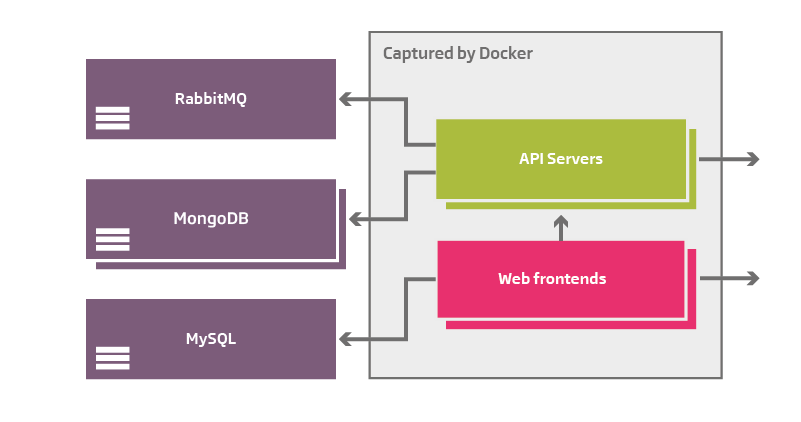
\includegraphics[width=0.4\textwidth]{images/docker-captures-data-free-parts.png}
    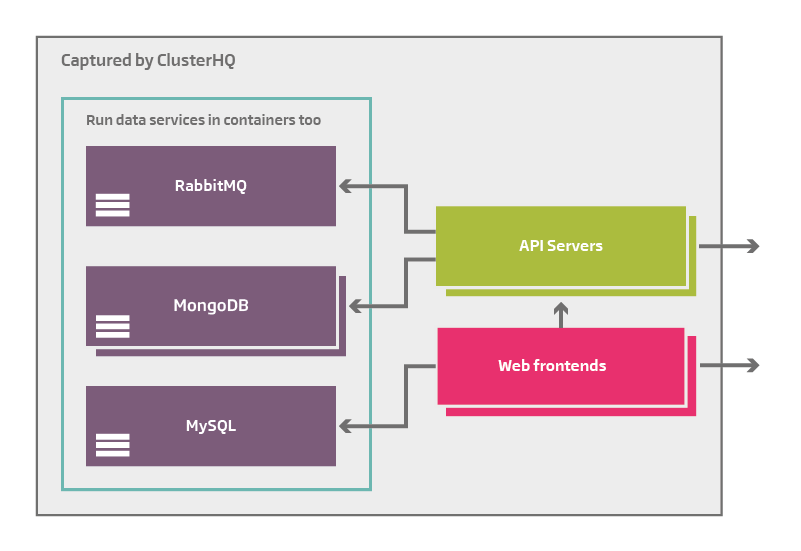
\includegraphics[width=0.4\textwidth]{images/clusterhq-captures-entire-app.png}
  }
  \caption{Individual Docker containers (left) compared to Flocker flock (right)}
  \label{fig:dockervsflocker}
\end{figure}


\begin{figure}[h!]
  \centering
  \makebox[\textwidth]{
    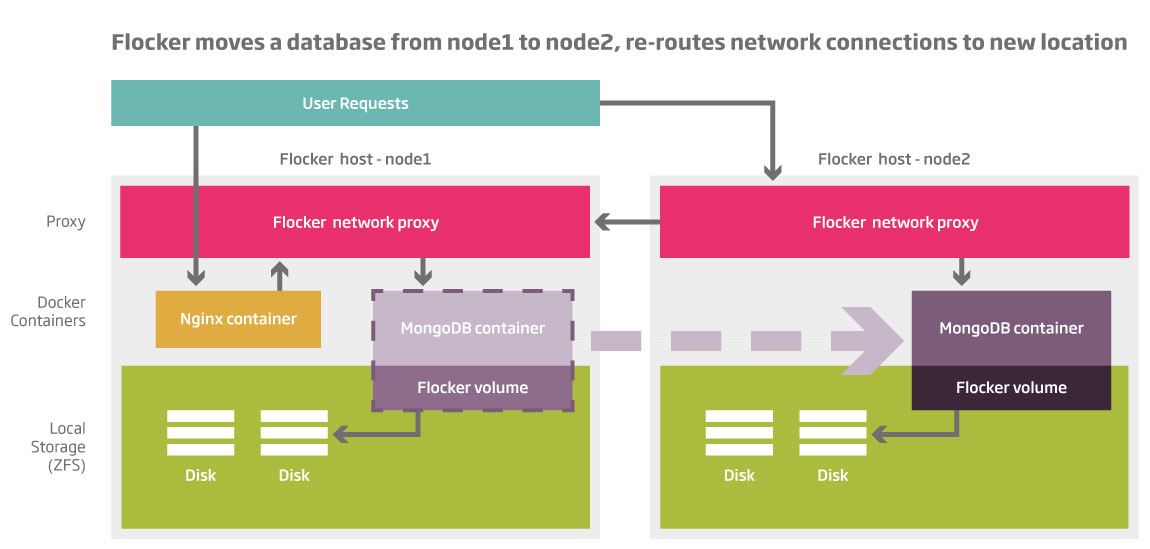
\includegraphics[width=0.7\textwidth]{images/flocker-architecture-diagram.jpg}
  }
  \caption{Flocker architecture diagram when moving (partial) containers}
  \label{fig:flockermovearchitecture}
\end{figure}


\pagebreak


\section{Goals}

\subsection{Research question}

\begin{framed}\begin{quote}{\Large Can we transparently migrate an application including data to where it is needed the most, and does this reduce latency?}\end{quote}\end{framed}

\subsection{Research question components}
\begin{itemize}
\item{Is application migration \textbf{feasible} using this setup?}
\item{Is migration of an application done \textbf{transparently}, and on which levels?}
\item{How long does migration take, and is this \textbf{delay} acceptable?}
\item{Can applications be migrated automatically based on \textbf{geographical shifts} of clients and does this \textbf{reduce latency}?}
\end{itemize}


\subsubsection{Test goals}
\begin{itemize}
  \item{\textbf{Goal 1:} Migrate instances between different VMs and servers.}
  \item{\textbf{Goal 2:} Migrate between different host OS (and perhaps localhost?)}
  \item{\textbf{Goal 3:} Measure user geo-distribution and migrate to localized server.}    
  \item{\textbf{Goal 4:} Generate global traffic with circadian cycle, and measure performance.}
  \item{\textbf{Optional goal:} Test this technique with a more complicated application like Diaspora \cite{diasporadocker} or OwnCloud \cite{ownclouddocker}.}
  \item{Test and create a simple working \textbf{module for Ansible} to manage Flocker as a proof-of-concept, and upload plugin to Github \cite{githubos3daffe}.}
\end{itemize}


\subsection{Questions/goals that are out of scope}
\begin{itemize}
\item{Scaling services based on load (static amount of containers)}
\item{Write entire management scripts to automate everything}
\item{Failure handling, to recover application when server crashes}
\item{Create vagrant test setup for east reproducing}
\item{Comparing performance to tradition replicated application}
\end{itemize}



\section{Ethical implications}
There are no apparent ethical implications since user data colletion is not required. All traffic will be automatically generated.



\section{Requirements}
We require several server instances in geographically remote locations for optimal testing. We intend to use several EC2 instances in conjunction with our SNE lab servers. We estimate the cost of the Amazon EC2 servers to be around \$40.



\begin{thebibliography}{99}
\bibitem{Docker}
\url{https://www.docker.com}
\bibitem{OSLV}
\url{http://www.ecsl.cs.sunysb.edu/tr/TR223.pdf}
\bibitem{whatisdocker}
\url{https://www.docker.com/whatisdocker/}
\bibitem{flocker}
\url{https://clusterhq.com}
\bibitem{flockerdoc}
\url{https://docs.clusterhq.com/en/0.3.2/}
\bibitem{ansible}
\url{http://www.ansible.com}
\bibitem{ansiblemod}
\url{http://docs.ansible.com/developing_modules.html}
\bibitem{elk}
\url{http://www.elasticsearch.org/overview/}
\bibitem{fig}
\url{http://www.fig.sh}
\bibitem{figgit}
\url{https://github.com/docker/fig}
\bibitem{foreman}
\url{http://theforeman.org}
\bibitem{foremandoc}
\url{http://theforeman.org/manuals/1.7/index.html}
\bibitem{vagrant}
\url{https://www.vagrantup.com}
\bibitem{diasporadocker}
\url{https://registry.hub.docker.com/u/chocobozzz/diaspora-docker/}
\bibitem{ownclouddocker}
\url{https://registry.hub.docker.com/u/jchaney/owncloud/}
\bibitem{githubos3daffe}
\url{https://github.com/OS3daffe/DAFFE}

\end{thebibliography}


\end{document}
